% !TEX root = ../../../main.tex
% 所属：第一部分：单变量分析学 / 第9章：一些不定积分的问题
% 节：9.1 不定积分的修正
% 正文按原文件顺序保存；由 ../chapter9.tex 调用。
\section{不定积分的修正}
\subsection*{常数修正}
也就是我们常常说的$+C$，与其他的教材不同的是，我们采取的是原函数的集合这一定义方式，所以常数修正在集合的意义下没有意义

这其实解释了很多初学者的疑惑，比如下面这个``悖论''：
\[
\int\frac{\dd x}{x}
=x\cdot \frac1x-\int x\cdot \dd\left(\frac1x\right)
=1+\int\frac{\dd x}{x},
\qquad\Longrightarrow\qquad 0=1.
\]
当然这并不是悖论，事实上\[0=1\equiv \{0+C:C\in \R\}=\{1+C:C\in\R\}\]

另外需要注意，只在结果后面装模作样地写上``$+C$（$C$ 是任意常数）''其实不一定能完成常数修正。这也是我们不再采用课本定义的原因。教材上的漏洞在修正体系下将被严肃对待.

\subsection*{``+C''的历史与实质}

在柯西（Cauchy）1823年的原始讲义中，不定积分的定义并非简单地``加一个任意常数''。柯西首先考虑了导数为零的函数：在连续情形下它可以被证明为常数，但在不连续情形下，它可能是\textbf{在每个连续区间上分别取不同常数值的函数}。因此，柯西定义的不定积分实际上是加了一个\textbf{函数}$\varphi(x)$，这个函数在每一个连续区间上恒为常数，但在不同区间上可以取不同的值。后续教材用字母 $C$ 代替 $\varphi(x)$ 作为简写，并强调``$C$ 不是一个固定不变的常数，也与 $x$ 的值无关''。

然而，这一精妙之处在代代相传中被简化成了``$+C$ 就是加任意常数''，丢掉了原定义最关键的细节。

\begin{figure}[H]
	\centering
	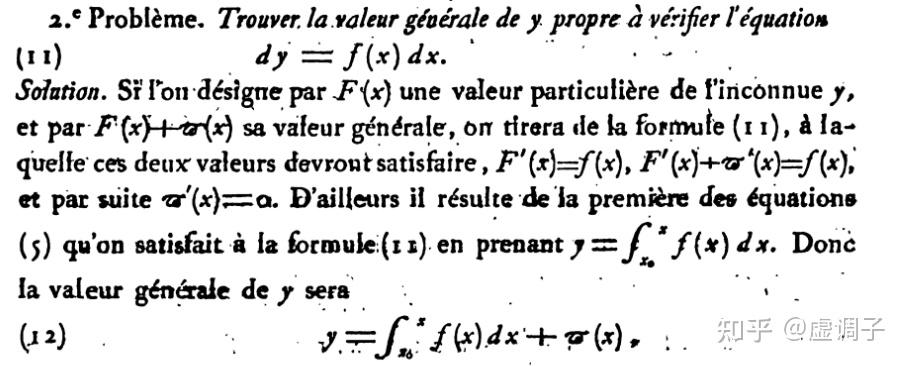
\includegraphics[width=0.85\linewidth]{figure/C9/005.jpg}
	\caption{柯西在1823年《无穷小分析讲义》中给出的不定积分定义：积分结果加上的是一个"函数"$\varphi(x)$，而非一个常数。}
\end{figure}

\begin{figure}[H]
	\centering
	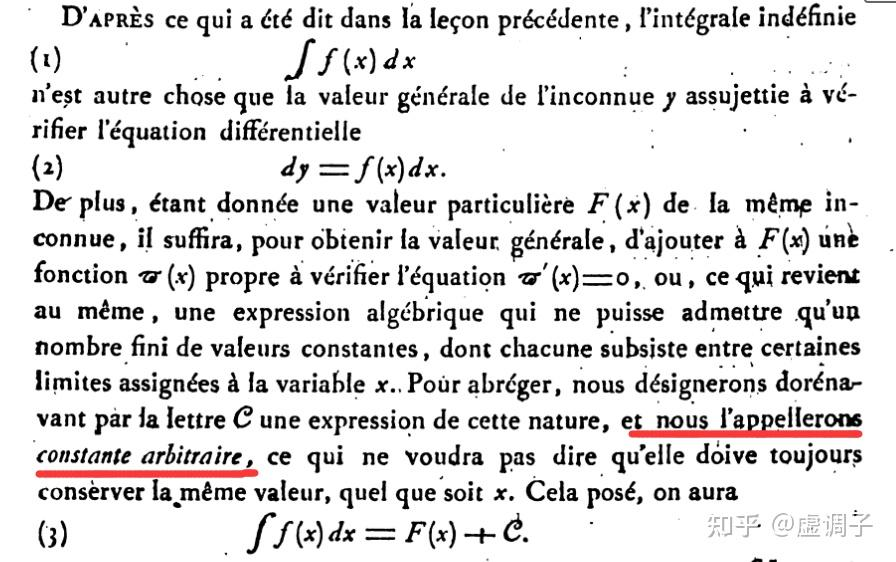
\includegraphics[width=0.85\linewidth]{figure/C9/007.jpg}
	\caption{柯西强调：用字母 $C$ 代替该函数只是简写，$C$ "不是一个固定不变的常数，也与 $x$ 的值无关"。}
\end{figure}

\begin{example}
	考虑 $\displaystyle\int\frac{\dd x}{x}$。常见答案 $\ln|x|+C$ 看似正确，实则不足。因为 $\frac1x$ 的定义域是 $(-\infty,0)\cup(0,+\infty)$，由两个不相连的区间组成。柯西定义下的真正结果是：

	\[
	\int\frac{\dd x}{x}=
	\begin{cases}
		\ln(-x)+C_1, & x<0,\\[4pt]
		\ln x+C_2,   & x>0,
	\end{cases}
	\]

	其中 $C_1$ 与 $C_2$ 是彼此独立的任意常数。仅写一个 $+C$ 会丢失一个自由度，因此在严格意义下是错误的。
\end{example}

\begin{figure}[H]
	\centering
	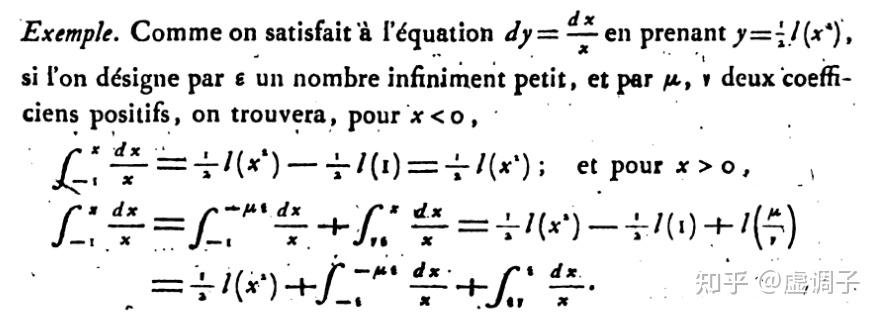
\includegraphics[width=0.85\linewidth]{figure/C9/009.jpg}
	\caption{柯西给出的 $\displaystyle\int\frac{\dd x}{x}=\frac12\ln(x^2)+\varpi(x)$，其中 $\varpi(x)$ 是各区间上独立的函数（现代记号写作 $\varphi(x)$ 或分段常数）。}
\end{figure}

\begin{example}
	更极端的情形出现在 $\displaystyle\int\frac{\dd x}{\cos^2x}$ 中。$\cos^2x$ 在 $x=\dfrac{\pi}{2}+k\pi$ 处为零，定义域被分割为无穷多个开区间：

	\[
	\int\frac{\dd x}{\cos^2x}=
	\begin{cases}
		\tan x+C_{-1}, & -\dfrac{3\pi}{2}<x<-\dfrac{\pi}{2},\\[6pt]
		\tan x+C_0,    & -\dfrac{\pi}{2}<x<\dfrac{\pi}{2},\\[6pt]
		\tan x+C_1,    & \dfrac{\pi}{2}<x<\dfrac{3\pi}{2},\\[6pt]
		\cdots
	\end{cases}
	\]

	此处需要\textbf{无穷多个}彼此独立的常数。这揭示了教科书公式表中 $\displaystyle\int\frac{\dd x}{\cos^2x}=\tan x+C$ 在严格意义下也是不完整的。
\end{example}

\subsection*{一个反例：传统$+C$导致的错误}

上述讨论并非咬文嚼字。在计算定积分时，若使用未经修正的不定积分公式，可能直接导致错误结果。

\begin{example}
	计算 $\displaystyle\int_0^{\pi}\frac{\dd x}{1+\sin^2x}$。

	采用传统公式
	\[
	\int\frac{\dd x}{1+\sin^2x}
	=\frac{1}{\sqrt2}\arctan\bigl(\sqrt2\tan x\bigr)+C,
	\]
	直接代入 Newton-Leibniz 公式：
	\[
	\int_0^{\pi}\frac{\dd x}{1+\sin^2x}
	=\left[\frac{1}{\sqrt2}\arctan\bigl(\sqrt2\tan x\bigr)+C\right]_0^{\pi}=0.
	\]

	但被积函数恒正，积分绝不可能为零。问题出在 $\tan x$ 在 $x=\dfrac{\pi}{2}$ 处间断，原函数在该点不连续，不能直接套用 Newton-Leibniz 公式。正确的做法是将积分区间在奇点处分段计算，或者使用经过\textbf{连续性修正}的结果（参见下文的连续修正方法），得到的真正结果是 $\dfrac{\pi}{\sqrt2}$。
\end{example}
\subsection*{$\operatorname{sgn}$ 与定义域修正}

由于开根号、去绝对值等操作会带来一个符号的差别，即原函数与所求得的表达式在定义域上相差一个符号，或者根据符号的需要缩小或扩大定义域，于是为了方便交流：
\begin{itemize}
	\item 后文将默认进行了对结果的 $\operatorname{sgn}$ 修正，变换过程省略。例如：
	\[
	\int \frac{\dd x}{x}=\ln(x)\bigl(=\ln|x|\bigr).
		\]
\end{itemize}


\begin{example}
	常用的
	\[
	\int \frac{\dd x}{1-x^2}=\operatorname{arth}x
	\]
	也可以认为默认进行了 $\operatorname{sgn}$ 修正。因为由 $\tanh x$ 的反函数来定义时，其定义域在 $|x|<1$。而不定积分的定义域要更广一些：
	\[
	\int\frac{\dd x}{1-x^2}=\operatorname{arth}x
	\left(=\frac12\ln\left|\frac{1+x}{1-x}\right|\right). 
	\]
	最直接的 $\operatorname{sgn}$ 修正就是利用 $\operatorname{sgn}()$ 函数解决。除此之外，取绝对值也是一种简单的 $\operatorname{sgn}$ 修正；对于复杂的函数将会有更复杂的修正结果。在追求结果的简洁和运算的简便方面，采用 $\operatorname{sgn}$ 修正是适合的。
	
	注意 $\operatorname{sgn}$ 修正不仅仅只有简单地添加符号，如
	\[
	\int\frac{\dd x}{1-x^2}
	=\frac12\operatorname{arth}\frac{2x}{1+x^2}. 
	\]
	相比 $\operatorname{arth}x$ 来说也是 $\operatorname{sgn}$ 修正，顺便将定义域扩大了。
\end{example}
\subsection*{连续性修正}
\begin{example}
	来尝试修正：
	\[
	\int\frac{\dd x}{1+\sin^2x}
	=\frac{1}{\sqrt2}\arctan\bigl(\sqrt2\tan x\bigr).
	\]
	原结果含有由 $\tan x$ 带来的间断。按照前面的思路，加上
	$x-\arctan(\tan x)$ 型的连续修正项，可得
	\[
	\begin{aligned}
		&\frac{1}{\sqrt2}\arctan\bigl(\sqrt2\tan x\bigr)
		-\frac{1}{\sqrt2}\arctan(\tan x)+\frac{x}{\sqrt2} \\
		&=\frac{1}{\sqrt2}\arctan
		\frac{(\sqrt2-1)\tan x}{1+\sqrt2\tan^2x}+\frac{x}{\sqrt2} \\
		&=\frac{1}{\sqrt2}\arctan
		\frac{(\sqrt2-1)\sin x\cos x}{\cos^2x+\sqrt2\sin^2x}+\frac{x}{\sqrt2} \\
		&=\frac{1}{\sqrt2}\arctan
		\frac{\sin 2x}{3+2\sqrt2-\cos 2x}+\frac{x}{\sqrt2}.
	\end{aligned}
	\]
	如图，由之前的间断函数变成了连续函数，连续修正成功。
\end{example}

\begin{figure}[H]
	\centering
	\begin{tikzpicture}[scale=0.75]
		\draw[gray!25, step=0.5] (-5,-2.2) grid (5,2.2);
		\draw[->] (-5.1,0)--(5.2,0) node[right] {$x$};
		\draw[->] (0,-2.25)--(0,2.35) node[above] {$y$};
		\foreach \x in {-4,-3,-2,-1,1,2,3,4}
		\draw (\x,0.05)--(\x,-0.05) node[below] {\scriptsize $\x$};
		\foreach \y in {-2,-1,1,2}
		\draw (0.05,\y)--(-0.05,\y) node[left] {\scriptsize $\y$};
		\draw[green!55!black, thick, domain=-4.6:-1.70, smooth, variable=\x]
		plot ({\x},{0.7071*rad(atan(1.4142*tan(\x r)))});
		\draw[green!55!black, thick, domain=-1.45:1.45, smooth, variable=\x]
		plot ({\x},{0.7071*rad(atan(1.4142*tan(\x r)))});
		\draw[green!55!black, thick, domain=1.70:4.6, smooth, variable=\x]
		plot ({\x},{0.7071*rad(atan(1.4142*tan(\x r)))});
		\node[green!55!black] at (-3.25,1.55)
		{$f(x)=\dfrac1{\sqrt2}\tan^{-1}(\sqrt2\tan x)$};
	\end{tikzpicture}
	\caption{不连续的结果}
\end{figure}

\begin{figure}[H]
	\centering
	\begin{tikzpicture}[scale=0.72]
		\draw[gray!25, step=0.5] (-6.5,-4.8) grid (6.5,2.5);
		\draw[->] (-6.6,0)--(6.7,0) node[right] {$x$};
		\draw[->] (0,-4.9)--(0,2.6) node[above] {$y$};
		\foreach \x in {-6,-5,-4,-3,-2,-1,1,2,3,4,5,6}
		\draw (\x,0.05)--(\x,-0.05) node[below] {\scriptsize $\x$};
		\foreach \y in {-4,-3,-2,-1,1,2}
		\draw (0.05,\y)--(-0.05,\y) node[left] {\scriptsize $\y$};
		\draw[green!55!black, thick, domain=-6.2:-4.85, smooth, variable=\x]
		plot ({\x},{0.7071*rad(atan(1.4142*tan(\x r)))});
		\draw[green!55!black, thick, domain=-4.55:-1.70, smooth, variable=\x]
		plot ({\x},{0.7071*rad(atan(1.4142*tan(\x r)))});
		\draw[green!55!black, thick, domain=-1.45:1.45, smooth, variable=\x]
		plot ({\x},{0.7071*rad(atan(1.4142*tan(\x r)))});
		\draw[green!55!black, thick, domain=1.70:4.55, smooth, variable=\x]
		plot ({\x},{0.7071*rad(atan(1.4142*tan(\x r)))});
		\draw[green!55!black, thick, domain=4.85:6.2, smooth, variable=\x]
		plot ({\x},{0.7071*rad(atan(1.4142*tan(\x r)))});
		\draw[red!70!black, thick, domain=-6.2:6.2, samples=220, smooth, variable=\x]
		plot ({\x},{0.7071*rad(atan(sin(2*\x r)/(3+2*sqrt(2)-cos(2*\x r))))+\x/sqrt(2)});
		\node[green!55!black] at (-4.45,0.85)
		{$f(x)=\dfrac1{\sqrt2}\tan^{-1}(\sqrt2\tan x)$};
		\node[red!70!black] at (-1.6,-4.15)
		{$g(x)=\dfrac1{\sqrt2}\tan^{-1}\!\left(\dfrac{\sin2x}{3+2\sqrt2-\cos2x}\right)+\dfrac{x}{\sqrt2}$};
	\end{tikzpicture}
	\caption{修正后连续的结果}
\end{figure}

\subsection*{反正切修正}

通常，经过一些粗暴的换元后，定义域已四分五裂。我们如果想要实现相应的修正，就需要一些特定的计算方法了。下面讨论一些对反正切函数的修正。注意，修正的思路不是唯一的。

\begin{example}
	对 $f(x)=\arctan(k\tan x)$ 进行连续性修正。
	
	前面的例题其实也已经提到，思路是加上 $x-\arctan(\tan x)$，即
	\[
	\begin{aligned}
		\arctan(k\tan x)
		&=\arctan(k\tan x)+x-\arctan(\tan x) \\
		&=x+\arctan\frac{(k-1)\tan x}{1+k\tan^2x} \\
		&=x+\arctan\frac{(k-1)\sin(2x)}{(k+1)-(k-1)\cos(2x)}.
	\end{aligned}
	\]
\end{example}

\begin{example}
	对
	\[
	f(x)=\arctan\left(k\left(x-\frac1x\right)\right)
	\]
	的修正。
	
	思路来源于魏念辉（$k\neq0$），
	\[
	\begin{aligned}
		\arctan\left(k\left(x-\frac1x\right)\right)
		&=\arctan\left(k\left(x-\frac1x\right)\right)
		+\arctan\left(\frac1{kx}\right)+\arctan(kx) \\
		&=\arctan\left(kx^3+\left(\frac1k-1\right)x\right)+\arctan(kx).
	\end{aligned}
	\]
	这样是在 $\R$ 上连续的函数了。
	
	另外，值得一提的是对于一般的
	\[
	\arctan\frac{Q_n(x)}{P_n(x)}
	\]
	有机械的思路修正。
\end{example}

\begin{proposition}
	\textbf{反正切修正公式.}
	若 $f(x)=i$ 有 $n$ 个复解 $x_k=a_k+i b_k$，那么
	\[
	\arctan f(x)=\sum_{k=1}^{n}\arctan\frac{x-a_k}{b_k}. 
	\]
	等号是修正意义下的。
\end{proposition}

\begin{proof}
	留意到 $\ln$ 与 $\arctan$ 的一些关系，
	\[
	\begin{aligned}
		\arctan f(x)
		&=\operatorname{Im}\bigl[\ln(1+i\cdot f(x))\bigr] \\
		&=\operatorname{Im}\left[\ln\left(i\prod_{k=1}^{n}(x-x_k)\right)\right] \\
		&=\operatorname{Im}\sum_{k=1}^{n}\ln(x-a_k-i b_k) \\
		&=\sum_{k=1}^{n}\arctan\frac{x-a_k}{b_k}.
	\end{aligned}
	\]
	其中整体的常数相位被纳入修正意义之中。由此可以把所有简单的且各间断点的反正切结果修正。
\end{proof}

\begin{example}
	由反正切修正公式可以得到
	\[
	\arctan\left(\frac{x^3-x^2-4x-1}{x^3+4x^2+x-1}\right)
	=\arctan x+\arctan(x+1)+\arctan(1+2x).
	\]
\end{example}

除此之外，我们还可以注意到一种反正切的修正，这类甚至改变了函数名。我们考虑
\[
\int\frac{\dd x}{a+x^2}
=\frac1{\sqrt a}\arctan\frac{x}{\sqrt a}\quad(a>0). \tag{1.21}
\]
这里会自动限制 $a$ 的范围，来源于符号的局限性。如果考虑 $a<0$，由前章导数表中 $\operatorname{arth}$ 的导数公式可得
\[
\int\frac{\dd x}{a+x^2}
=-\frac1{\sqrt{-a}}\operatorname{arth}\frac{x}{\sqrt{-a}}\quad(a<0). 
\]
这两者在考虑复数域后是一致的，可以作为一种定义域修正处理。在后文中，如果 $a$ 的符号未知，那么我们采用 $\arctan$ 形式而省略定义域修正，以避免一些无聊的讨论。

如果考虑 $a=0$ 时，上式需要更进一步的修正，使得 $a$ 对于趋近极限过程连续。对于 $a>0$，也可以写成
\[
\int\frac{\dd x}{a+x^2}
=-\frac1{\sqrt a}\arctan\frac{\sqrt a}{x}\quad(a>0). 
\]
这样取极限都会有
\[
\int\frac{\dd x}{x^2}=-\frac1x. 
\]

\subsection*{取整函数的修正}

取整函数是指 $f(x)=[x]$，输出不超过 $x$ 的最大整数。由于分别在每个区域都是常数，所以取整函数的不定积分核心就是修正。

思路是采用多项式法。例如：
\[
\int [x]\dd x=x[x]+P_2([x])=x[x]-\frac12[x](1+[x]). 
\]
日常生活中，我们可能还会遇到小数部分函数，也即
\[
f(x)=\{x\}=x-[x]\geq0. 
\]
它们组合的更复杂的积分也可以利用多项式法修正，这里不详细展开，只举一个高次的例子：
\[
\int x\{x\}[x]\dd x
=\frac12x^2\{x\}^2-\frac23x\{x\}^3
+\frac16\{x\}^3+\frac13[x]^3+\frac16[x]^2. 
\]




